\section[Selecci\'on $\nu$]{Selecci\'on de neutrinos}

\begin{frame}
 \frametitle{Estrategia de cada b\'usqueda}
 \begin{center}
  \pgfimage[width=0.9\textwidth]{./fig/estrategiaAuger/analysisSchema_3}
 \end{center}
\end{frame}

\begin{frame}{Selecci\'on de eventos de calidad}
\begin{block}{Eliminaci\'on de:}
 \begin{enumerate}[<alert@+|+->]
  \item PMT defectuosos o con se\~nales espureas
  \item Se\~nales debidas a muones accidentales
  \item Estaciones aisladas espacial o temporalmente
 \end{enumerate}
\end{block}

\begin{exampleblock}{Ejemplo:}
 \begin{overprint}
 \onslide<1>\centerline{\includegraphics[width=0.48\textwidth]{fig/seleccionAuger/pmt2_border}\hspace*{2mm}
 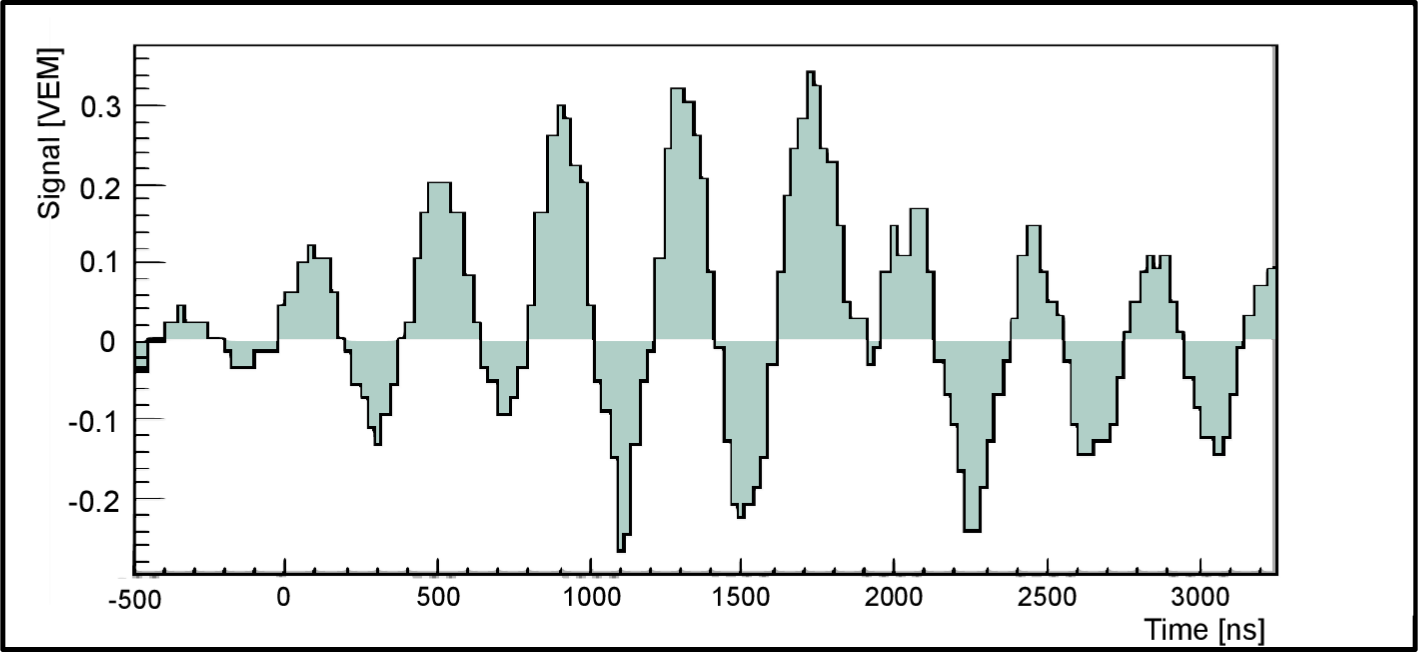
\includegraphics[width=0.48\textwidth]{fig/seleccionAuger/lighting}}
 \onslide<2>\centerline{\includegraphics[height=0.35\textwidth]{fig/seleccionAuger/badStartTime_2}}
 \onslide<3>\centerline{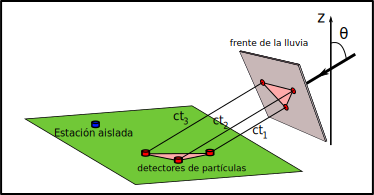
\includegraphics[height=0.35\textwidth]{fig/seleccionAuger/geome2}}
 \end{overprint}
\end{exampleblock}
\end{frame}


\begin{frame}
\frametitle<1>{Selecci\'on de lluvias inclinadas: Huella elongada}
\frametitle<2->{Selecci\'on de lluvias inclinadas: Informaci\'on temporal}
	\begin{center}
		\begin{textblock}{6.5}(0.4,3)
% 			\begin{block}{Variables:}
			\begin{overprint}
			\onslide<1>\centerline{\pgfimage[width=1.0\textwidth]{fig/seleccionAuger/L_W_0.pdf}}
			\onslide<2->\centerline{\pgfimage[width=1.0\textwidth]{fig/seleccionAuger/L_W.pdf}}
			\end{overprint}
% 			\end{block}
		\end{textblock}
		
		\begin{textblock}{8.1}(7.4,2.5)
% 			\begin{alertblock}{}
			\begin{overprint}
			\onslide<1>\centerline{\pgfimage[height=0.65\textwidth]{fig/seleccionAuger/huellas}}
			\onslide<2->\centerline{\pgfimage[height=0.65\textwidth]{fig/seleccionAuger/sigSpeed2}}

% 			\onslide<2>
% 				\begin{tabular}{c c}
% 				Lluvia vertical & Lluvia horizontal\\
% 				$ \Delta T_{ij}\approx 0 \rightarrow V\gg c$ &$ V \approx c$\\
% 				\end{tabular}
% 				\pgfimage[width=\textwidth]{fig/seleccionAuger/sigSpeed.pdf}
			\end{overprint}
% 			\end{alertblock}
		\end{textblock}
		\begin{textblock}{15}(0.5,10.0)
			\begin{exampleblock}{}<3>
			\renewcommand{\arraystretch}{1.4}
			\scriptsize
			\centering
			\begin{tabular}{|l|c|c|c|}
			\hline
			Búsqueda & Earth-skimming (ES)           & Downward-going                        & Downward-going                       \\
					&                               & {\it high} angle (DGH)                & {\it low} angle (DGL)                \\
			\hline
						& $-$                             & $\theta_{\rm rec}>$ 75$^{\circ}$   &   $\theta_{\rm rec}\in (58.5^\circ,~76.5^{\circ})$\\
			Lluvias    & $L/W > 5$                                         & $L/W > 3$ & $-$ \\
			Inclinadas & $\langle V\rangle\in (0.29,~0.31)~{\rm m~ns^{-1}}$ & $\langle V \rangle~<~0.313~{\rm m~ns^{-1}}$ & $-$ \\
					& RMS($V$)$~<~0.08~{\rm m~ns^{-1}}$                 & RMS($V$)/$\langle V\rangle<0.08$ & $-$ \\
					& Conf 1 si $N_{ST}=3$ & & \\
			\hline
			\end{tabular}
			\end{exampleblock}
		\end{textblock}
	\end{center}
\end{frame}

\begin{frame}
\frametitle<1>{Selecci\'on de lluvias j\'ovenes: Time over Threshold (ToT)}
\frametitle<2>{Selecci\'on de lluvias j\'ovenes: Area over Prak (AoP)}
\frametitle<3>{Selecci\'on de lluvias j\'ovenes}
	\begin{center}\footnotesize
		
		\begin{textblock}{15}(0.5,2)
			\begin{alertblock}{}
				\begin{overprint}
				\onslide<1>\centerline{\textbf{13 bines temporales sobre umbral.}}
				\onslide<2->\centerline{\textbf{\'Area de la se\~nal dividido su m\'aximo.}}
				\end{overprint}
			\end{alertblock}
		\end{textblock}

		
		\begin{textblock}{7.3}(0.4,3.5)
			\begin{block}{Se\~nal extendida}
			\centerline{\pgfimage[width=0.8\textwidth]{fig/seleccionAuger/traza_tot_m}}
			\begin{overprint}
			 \onslide<1>\centerline{\textbf{Disparo ToT}}
			 \onslide<2->\centerline{\textbf{AoP grande}}
			\end{overprint}
			\end{block}
		\end{textblock}
		
		\begin{textblock}{7.3}(8.3,3.5)
			\begin{block}{Se\~nal angosta}
			\centerline{\pgfimage[width=0.8\textwidth]{fig/seleccionAuger/traza_t2_m}}
			\begin{overprint}
			 \onslide<1>\centerline{\textbf{Disparo No ToT}}
			 \onslide<2->\centerline{\textbf{AoP peque\~no}}
			\end{overprint}
			\end{block}
		\end{textblock}
		
		\begin{textblock}{15}(0.5,10.0)
			\begin{exampleblock}{}<3>
				\begin{center}
					{\scriptsize
					\renewcommand{\arraystretch}{1.3}
						\begin{tabular}{|c|c|c|}
						\hline
						Earth-Skimming (ES)          & Down-going High (DGH)    & Down-going Low (DGL)                       \\
						\hline\hline
						Data: 1 enero 04 - 31 mayo 10 &                                      & $\geq 75\%$ de las estaciones cerca \\
						$\geq 60\%$ de las estaciones con  &                                      & del core con ToT trigger  \\
						ToT trigger \& AoP $>$ 1.4    & Discriminante de Fisher basado             &      \&                      \\
						\cline{1-1}
						Data: 1 junio 10 - 20 junio 2013   & en AoP de estaciones tempranas & Discriminante de Fisher basado  \\
						$\langle {\rm AoP} \rangle> 1.83$  &                                 &  en el AoP de las estaciones \\
						AoP$_{\rm min}$ $>$ 1.4 if Nst=3   &                                 & tempranas cercanas al core         \\
						\hline
						\end{tabular}
					}
				\end{center}
			\end{exampleblock}
		\end{textblock}
	\end{center}
\end{frame}

\begin{frame}
 \frametitle{Selecci\'on de lluvias j\'ovenes}
 \framesubtitle{Ejemplo: AoP promedio (an\'alisis ES)}
	\begin{center}
	\pgfimage[width=0.9\textwidth]{fig/seleccionAuger/AoP_new_without_search_0.pdf}<1>
	\pgfimage[width=0.9\textwidth]{fig/seleccionAuger/AoP_new_without_search_2.pdf}<2>
	\pgfimage[width=0.9\textwidth]{fig/seleccionAuger/estimaBackground.pdf}<3>
	\pgfimage[width=0.9\textwidth]{fig/seleccionAuger/AoP_new_without_search_1.pdf}<4->
	\end{center}
	
	\begin{textblock}{4.3}(7.3,8.5)
		\begin{alertblock}{}<only@4>
		\centering
	         Eficiencia de selecci\'on $\sim 90\%$	
		\end{alertblock}
	\end{textblock}
	
\end{frame}

